\apendice{Detalhes do método e dos dados}{ap:metodo}

\textit{O que contém:} a construção da matriz do lote, a implementação do Húngaro, as fontes e regras de construção dos dados reais, a geografia dos cenários sintéticos e os procedimentos estatísticos. \textit{Quando consultar:} para conferir como a decisão de cada lote é calculada e como as entradas da simulação foram montadas.

\apendicesubtitulo{Matriz do lote}

Para resolver a equação~\ref{art-eq:obj} com um único problema de atribuição, constrói-se uma matriz ampliada com uma linha por pedido pendente e colunas para os veículos mais $|R_t|$ colunas fictícias de \enquote{não atribuído}. O elemento de um par elegível é $c_{rv}-M$, o de um par inelegível é um valor proibitivo e o de uma coluna fictícia é zero. Com $M$ maior que a soma de qualquer conjunto de custos ($M=\max c\,(|R_t|+1)+1$), todo par adicional baixa o custo total, de modo que o número de atendidos domina e o custo de aproximação desempata. Os custos são inteiros (metros multiplicados por $10^5$, somados a um índice de posição), o que torna o desempate determinístico. A matriz é retangular, mas, como há pelo menos tantas colunas quanto linhas, o método se aplica sem alteração.

\apendicesubtitulo{Implementação do Húngaro}

A implementação usa dois vetores de potenciais (um por linha e um por coluna) e insere um pedido por vez. Para cada pedido, calcula a menor folga de cada coluna ainda não visitada, desloca os potenciais por essa folga (o que mantém os custos reduzidos não negativos e nulos nos pares escolhidos) e inverte o caminho aumentante até uma coluna livre. É o método primal-dual de \citeonline{kuhn1955} e \citeonline{munkres1957} organizado como sequência de caminhos mínimos com potenciais \cite{tomizawa1971, edmondskarp1972}, em $O(n^2 m)$ para $n$ linhas e $m$ colunas; não há enumeração nem programação linear. A rotina de atribuição da biblioteca SciPy, que usa busca de caminho aumentante no estilo de \citeonline{jonker1987} e atribuições retangulares \cite{crouse2016}, serviu apenas de referência em testes, para comparar o número de pares e a soma das distâncias, e não a identidade dos pares. Os testes usam enumeração exaustiva em instâncias de até $4\times4$, comparação com o SciPy em instâncias maiores e conferência de 2.628 lotes reais de desenvolvimento. A otimalidade assegurada é a de cada lote, não a do dia. Empates entre soluções de mesmo custo são resolvidos pelo índice determinístico. A Figura~\ref{fig:fluxo} resume o fluxo de um lote.

\begin{figure}[!htb]
\caption{Fluxo da atribuição em lote}\label{fig:fluxo}
\centering
\begin{tikzpicture}[node distance=7mm, box/.style={draw, rounded corners=2pt, align=center, font=\fontsize{9}{10}\selectfont, minimum height=10mm, text width=34mm}, >=Stealth]
\node[box](a){Instante de lote $t$ (múltiplo de 60 s)};
\node[box,right=of a](b){Pedidos pendentes (chegada $\le t$)};
\node[box,right=of b](c){Veículos elegíveis (livres, no raio, sem conflito)};
\node[box,below=of c](d){Matriz de custos $c_{rv}$ (km)};
\node[box,left=of d](e){Escolha: lote sequencial ou atribuição conjunta};
\node[box,left=of e](f){Validação: pares únicos e elegíveis};
\node[box,below=of f](g){Atualização de ocupação, posição e liberação};
\node[box,right=of g](h){Pedidos sem par seguem para $t+60$ s};
\draw[->](a)--(b);\draw[->](b)--(c);\draw[->](c)--(d);\draw[->](d)--(e);\draw[->](e)--(f);\draw[->](f)--(g);\draw[->](g)--(h);
\end{tikzpicture}
\par\fonte{elaborada pelos autores a partir do simulador.}
\end{figure}

\apendicesubtitulo{Fontes dos dados reais}

As entidades foram extraídas do banco operacional (SQL Server) e do índice de posições de ofertas (Elasticsearch). As posições dos veículos ofertados são instantâneos a cada cerca de 2 minutos; o cadastro de veículos é uma fotografia única extraída em 08/11/2026. A telemetria de terceiros existe só em fevereiro e março e \textbf{não} é usada: nenhuma quilometragem do estudo é odométrica ou validada por ela. Os arquivos derivados são armazenados em Parquet com manifesto e SHA-256 por dia; a extração depende de consultas somente leitura e não de plataformas em nuvem.

\apendicesubtitulo{Regras de construção}

todas fixadas antes da execução congelada:
\begin{alineas}
\item \textit{Elegibilidade do dia}: entidades do dia presentes, ao menos 300 instantes de posição e ao menos 200 pedidos; os 15 dias de setembro e os 25 de outubro cumpriram (mínimos de 702 instantes e 459 pedidos), sem exclusão.
\item \textit{Disponibilidade}: a presença de um veículo no registro de ofertas não prova disponibilidade, pois esse registro inclui veículos ocupados e subcobre parte da atividade. A janela de um motorista é a jornada registrada interseccionada com a presença no registro, estendida por lacunas de até 1.200 s; lacunas maiores ficam como desconhecidas e fora da janela; compromissos externos bloqueiam o motorista. A jornada usada é a realizada, informação disponível só retrospectivamente ao avaliador, comum a todas as políticas.
\item \textit{Posição inicial}: primeira posição observada do motorista na janela. Depois disso, ocupação e posição vêm das corridas que o próprio simulador atribui; as corridas históricas não entram como compromissos.
\item \textit{Parâmetros}: fator rua/reta de 1,3012 e velocidade de aproximação de 16,079 km/h, estimados na calibração de março com as distâncias de aproximação registradas pelo aplicativo em um extrato anterior dos mesmos dados (466 aproximações); raio de despacho de 4,5 km em linha reta e paciência de 180 s, ajustados naquela calibração para reproduzir o aceite e o tempo de busca observados (janela das 4 às 11 h).
\item \textit{Duração das viagens}: a duração de cada corrida com passageiro é a observada (na falta, a mediana do dia); não depende do modelo de distância.
\item \textit{Tentativas}: novas solicitações do mesmo passageiro em pouco tempo não foram deduplicadas, e cancelamentos posteriores à atribuição não são modelados.
\item \textit{Privacidade}: identificadores pseudonimizados por HMAC-SHA256 com segredo fora do repositório; só agregados são reportados.
\end{alineas}

O número de motoristas por dia caiu de 106,8 no treino para 74,3 em outubro; a queda aparece também nos motoristas distintos com corrida encerrada (108,4 e 70,4) e na demanda (1.207 e 941 pedidos por dia). As três séries são compatíveis com mudança da operação, mas não excluem alterações de registro ou recorte. Jornadas registradas com vínculo ambíguo (placa associada a vários motoristas no dia, de 36 a 47 por dia) não delimitam a janela, que passa a vir só do registro de ofertas. A Tabela~\ref{tab:info} separa o que a política pode saber do que só o avaliador sabe.

\begin{table}[!htb]
\caption{Planos de informação nos dados reais}\label{tab:info}
\centering\fontetabela
\begin{tabular}{|p{34mm}|p{62mm}|p{52mm}|}
\hline
\textbf{Plano} & \textbf{Conteúdo} & \textbf{Disponível à política?} \\
\hline
Política (instante $t$) & pedidos chegados até $t$; veículos online, livres e elegíveis em $t$; distâncias estimadas & sim \\
\hline
Ambiente retrospectivo & janelas de jornada realizadas, presença no registro de ofertas, compromissos externos, cadastro de veículos & não: reconstruídos com o dia completo; iguais nas três políticas \\
\hline
Hipóteses de simulação & raio, velocidade, fator rua/reta, paciência, posição inicial, ausência de aceite e de cancelamento pós-atribuição & não: parâmetros fixos, herdados de março \\
\hline
\end{tabular}
\fonte{elaborada pelos autores a partir da documentação do experimento.}
\end{table}

\apendicesubtitulo{Fator rua/reta e escolha}

O km é estimado (distância em linha reta vezes 1,3012), não medido por odômetro. Como o raio e os custos do lote usam a distância em linha reta, o fator não altera a escolha em um lote fixo: multiplicar todos os custos por uma constante positiva preserva a ordenação e o ótimo da atribuição. O fator muda, porém, o km contabilizado e o tempo de aproximação, e portanto a ocupação dos veículos e a evolução do dia; quando há limites associados à distância, como um raio medido por via, muda também quem é elegível.

\apendicesubtitulo{Geografia dos cenários sintéticos}

O instantâneo do OpenStreetMap é o da consulta à API Overpass (versão 0.7.62.11) de 08/11/2026, às 15:13 UTC, com 36.350 elementos de via, licença ODbL; a malha do IBGE usa o sistema WGS84 (EPSG:4326); ambos foram registrados com SHA-256. Pontos de parada são nós viários, um por célula H3 de resolução 8, a no máximo 20 km por via, ida e volta, do centro de Vitória. As células H3 servem só para escolher os pontos de parada e definir as zonas do gerador de demanda (e para o mapa); não participam da atribuição. A Figura~\ref{fig:mapa} mostra que o recorte (75 células e 368 pontos de parada) cobre a ilha de Vitória e partes de Vila Velha, Cariacica e Serra, e não toda a região metropolitana; é um recorte experimental, não um limite administrativo nem a área de atuação de uma empresa.

\begin{figure}[!htb]
\caption{Recorte geográfico dos cenários sintéticos: células H3 de resolução 7 com pontos de parada}\label{fig:mapa}
\centering
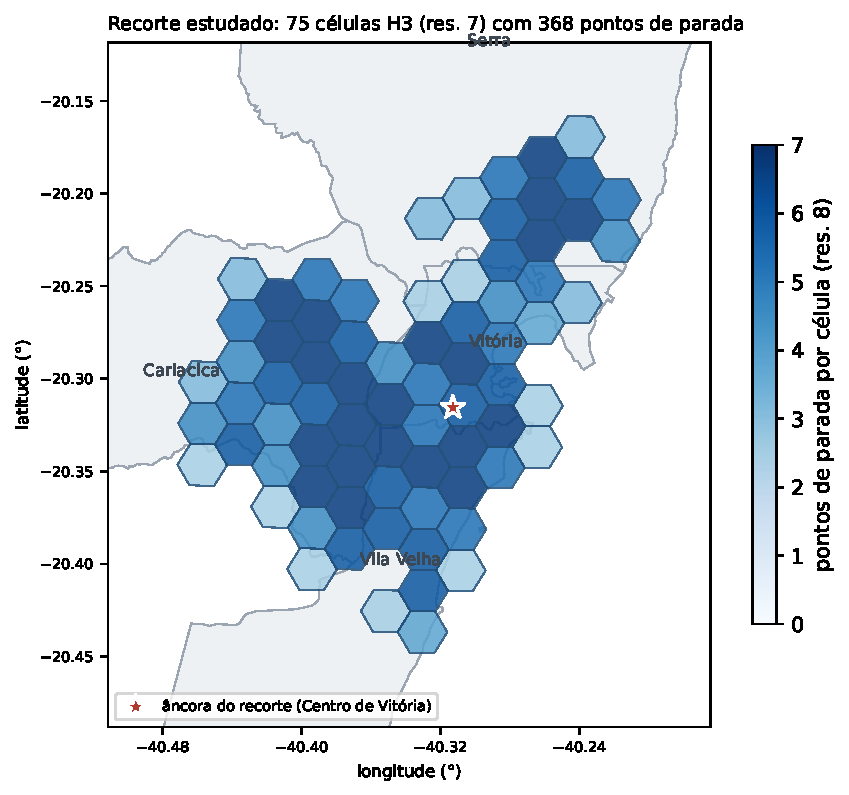
\includegraphics[width=0.7\linewidth]{figures/study_area_h3_map_no_footer.pdf}
\par\fonte{Elaboração própria com dados do IBGE e OpenStreetMap (ODbL).}
\end{figure}

O arquivo do OpenStreetMap contém 521 trechos marcados como ponte ou viaduto, entre eles a Ponte Deputado Darcy Castello de Mendonça, a Ponte Governador Gerson Camata, a Ponte do Príncipe e a Ponte Florentino Avidos. As verificações feitas foram estruturais: o grafo do recorte é conexo (as distâncias entre os 368 pontos são todas finitas), a distância por via nunca é menor que a distância em linha reta, e a razão entre as duas, em mediana, é de 1,45 entre Vitória e Vila Velha e de 1,34 dentro de Vila Velha, de modo que há travessia mapeada entre a ilha e o continente. \textbf{Não} se verificou ponte a ponte se cada ligação existente está mapeada nem se validaram tempos de percurso contra medições; não se afirma, portanto, que as pontes estejam corretamente representadas, e congestionamento e travessias bloqueadas não são modelados.

\apendicesubtitulo{Gerador e variantes}

O gerador (versão 1.0.0) tem parâmetros registrados; as jornadas de 9 horas começam às 6, 8, 10 ou 12 h. Velocidade, raio e paciência são hipóteses para uma operação sintética, não calibradas. Das 17 variantes, quatro alteram a relação frota/demanda (4 ou 14 pedidos por veículo, contra 8), quatro alteram a resolução das zonas do gerador de demanda e nove alteram só parâmetros de um planejador de reposicionamento que não participa do despacho; estas nove são novos sorteios do cenário-base (o código do cenário entra na semente), e não condições diferentes. As concentrações de demanda são hipóteses e não representam padrões reais. As sementes finais (20001--20040) foram reservadas antes da execução; as de desenvolvimento (101--120) foram usadas antes.

\apendicesubtitulo{Estatística}

Nos dados reais, o custo de cada par é $c_{rv}=1{,}3012\,h_{rv}$, com $h_{rv}$ a distância em linha reta. Nos cenários sintéticos, $c_{rv}$ é a distância por via, sem esse fator. A diferença em km é $\Delta K = K_C - K_{ref}$. A variação relativa aos atendidos da referência, $100\,\Delta N/N_{ref}$, é outra quantidade que a diferença em pontos percentuais e é identificada como tal quando citada. A espera de um pedido atendido é o tempo entre a chegada e o despacho mais o deslocamento estimado até a origem. Uma política que atende pedidos que a outra deixa expirar pode ter espera média maior ou menor por esse motivo, e a espera não é, por si só, evidência de melhora do serviço. O IC95\% da média das diferenças diárias usa \textit{bootstrap} de blocos móveis circulares de 7 dias (10.000 reamostragens, semente 20261108), que respeita a dependência temporal entre dias; a sensibilidade desse intervalo está no Apêndice~\ref{art-ap:repro} (Tabela~\ref{tab:ic}). Três perguntas são distintas: se o critério de atendimento foi cumprido (contagem no período); se a diferença é distinguível de zero (intervalo); e se as políticas são equivalentes, ou a atribuição conjunta não inferior ao despacho imediato, dentro de uma margem. Um intervalo que inclui zero responde à segunda, não à terceira. A terceira exige uma margem justificada por critério externo ou operacional; nenhuma foi fixada antes, e nenhuma é definida agora, para não escolher a margem à luz da perda observada. Nos cenários sintéticos, os 20 testes previstos no plano (5 cenários principais $\times$ 4 variantes de despacho em lote avaliadas no experimento, contra o despacho imediato: 20 testes) usam correção de Holm, e os resultados sintéticos são interpretados como exploratórios, pois já eram conhecidos na decisão de adotar o método. Totais por período e diferença média diária são ambos reportados; os totais respondem pela soma de km, e os intervalos, pela variação entre dias.

\apendice{Verificações, análises posteriores e reprodutibilidade}{ap:repro}

\textit{O que contém:} as verificações do congelamento, as diferenças diárias dos dados reais, os intervalos alternativos, a sensibilidade, a recalibração com o teste fora da amostra, os valores absolutos do guloso global e a conferência da coleta. \textit{Quando consultar:} para conferir de onde vem cada número de \nameref{art-sec:resultados} e quão estável ele é.

Antes de simular setembro e outubro, congelaram-se: o SHA-256 do código (151 arquivos do pacote e dos \textit{scripts} da avaliação), \texttt{480a98a1\ldots e93f87}; o \textit{commit} de base \texttt{3e77cb9}; a versão do Python (3.12.14); 201 manifestos de dados com SHA-256, todos conferidos contra os arquivos Parquet; e a configuração das três políticas. Testes automáticos no congelamento (código anterior à reorganização): 535 aprovados e 1 pulado; análise estática sem erros. Verificações em quatro dias de desenvolvimento (10/02, 04/03, 17/03 e 25/03): em 2.628 lotes, o Húngaro coincidiu com o oráculo em número de pares e soma de distâncias (resolução de 1 m); todos os pedidos de cada lote já haviam chegado na decisão; decisões apenas em múltiplos de 60 s; pares únicos e elegíveis; nenhuma sobreposição de serviços por motorista; o lote sequencial (B) coincide com uma reimplementação independente. Nos períodos finais: 15 de 15 e 25 de 25 dias elegíveis; 19 (setembro) e 17 (outubro) compromissos com posição de entrada inconsistente, independentes da política e iguais nas três. Após a avaliação, o código foi reorganizado em novos módulos (o hash do código atual difere do congelado, e os manifestos antigos não foram reescritos). A equivalência foi conferida por reexecução de amostras: três pares (cenário, semente) sintéticos e um dia real reproduziram os resultados congelados, e a análise regenerada dos arquivos congelados reproduziu as tabelas dos dois períodos; essas reexecuções não são novos testes científicos. Depois dos resultados, a reexecução das três políticas sobre as entradas congeladas, com o código reorganizado, reproduziu os 120 resultados (dia e política) de setembro e outubro, e a reconstrução das entradas pelo código atual reproduziu os totais dos dois períodos. Sobre a rede viária dos cenários sintéticos, as verificações foram estruturais (grafo conexo, distância por via não inferior à reta, razão ilha--continente comparável à interna) e não incluem validação de tempos de percurso nem conferência ponte a ponte.

\figura[0.95\linewidth]{figures/empty_km_service_differences.pdf}{Variação de km vazio e de atendimento entre despacho imediato (A), lote sequencial (B) e atribuição conjunta (C), por período (dados reais, calibração de março)}{Elaboração própria com resultados congelados; comparação de C com A e B.}{fig:km}

A Tabela~\ref{tab:diario} traz as diferenças diárias pareadas dos dados reais, e a Tabela~\ref{tab:ic}, a sensibilidade do intervalo de confiança da média diária ao tamanho do bloco e a um intervalo $t$ pareado. Com 15 dias, blocos de 7 dias deixam só três blocos por reamostragem, e o intervalo de setembro fica mais estreito que os demais; o limite superior para km fica abaixo de zero em todas as variantes, e, para atendidos C×A, todos os intervalos incluem zero.

\begin{table}[!htb]
\caption{Diferenças diárias da atribuição conjunta (C) contra o despacho imediato (A) e o lote sequencial (B), agrupadas por semana (dados reais, calibração de março)}\label{tab:diario}
\centering\fontetabela\setlength{\tabcolsep}{5pt}
\begin{tabular}{|l|r|r|r|r|}
\hline
 & \multicolumn{2}{|c|}{\textbf{Contra o despacho imediato}} & \multicolumn{2}{|c|}{\textbf{Contra o lote sequencial}} \\
\hline
\textbf{Dia} & \textbf{\shortstack{Diferença de\\km vazio (km)}} & \textbf{\shortstack{Diferença de\\atendidos}} & \textbf{\shortstack{Diferença de\\km vazio (km)}} & \textbf{\shortstack{Diferença de\\atendidos}} \\
\hline
\multicolumn{5}{|l|}{\textit{Setembro}} \\
\hline
16/09 qua & −108,6 & +36 & −22,7 & +67 \\
\hline
17/09 qui & −224,3 & +13 & −106,0 & +13 \\
\hline
18/09 sex & −204,2 & +10 & −121,7 & −3 \\
\hline
19/09 sáb & +4,0 & +12 & −35,6 & +8 \\
\hline
20/09 dom & −33,4 & −13 & −12,6 & +6 \\
\hline
21/09 seg & −75,4 & −12 & −40,1 & −13 \\
\hline
22/09 ter & −122,4 & −8 & −26,4 & +19 \\
\hline
23/09 qua & −155,1 & +25 & +1,2 & +71 \\
\hline
24/09 qui & −257,6 & −31 & −146,7 & −17 \\
\hline
25/09 sex & −160,1 & +3 & −130,9 & +6 \\
\hline
26/09 sáb & −24,6 & −15 & −10,1 & +9 \\
\hline
27/09 dom & −23,3 & +4 & −17,4 & −6 \\
\hline
28/09 seg & −134,8 & +1 & −55,0 & +5 \\
\hline
29/09 ter & −124,3 & −10 & −25,8 & +19 \\
\hline
30/09 qua & −123,1 & +1 & −33,8 & +7 \\
\hline
\multicolumn{5}{|l|}{\textit{Outubro}} \\
\hline
01/10 qui & −152,9 & −19 & −65,3 & 0 \\
\hline
02/10 sex & −162,7 & +16 & −69,6 & +14 \\
\hline
03/10 sáb & −104,0 & +8 & −35,4 & +31 \\
\hline
04/10 dom & −50,4 & −3 & −7,8 & +4 \\
\hline
05/10 seg & −149,2 & −33 & −44,1 & 0 \\
\hline
06/10 ter & −65,9 & +31 & −18,6 & +37 \\
\hline
07/10 qua & −88,4 & −8 & +22,5 & +1 \\
\hline
08/10 qui & −143,5 & −9 & +5,9 & −11 \\
\hline
09/10 sex & −124,9 & −18 & −24,6 & +11 \\
\hline
10/10 sáb & −58,3 & −13 & +5,5 & +11 \\
\hline
11/10 dom & −73,8 & +3 & −63,2 & +6 \\
\hline
12/10 seg & −25,4 & −4 & +14,6 & +4 \\
\hline
13/10 ter & −38,5 & −10 & +10,3 & +10 \\
\hline
14/10 qua & −9,6 & −1 & +23,3 & −4 \\
\hline
15/10 qui & −133,8 & +32 & −101,2 & +27 \\
\hline
16/10 sex & −78,2 & −2 & −9,5 & −3 \\
\hline
17/10 sáb & −82,0 & −11 & −28,4 & −4 \\
\hline
18/10 dom & −21,6 & +2 & −4,0 & +8 \\
\hline
19/10 seg & −85,7 & −37 & −30,2 & −15 \\
\hline
20/10 ter & −84,5 & −4 & −65,7 & +11 \\
\hline
21/10 qua & −79,4 & −29 & −61,1 & −21 \\
\hline
22/10 qui & −72,9 & 0 & +27,0 & +11 \\
\hline
23/10 sex & −22,1 & +17 & +24,8 & +6 \\
\hline
24/10 sáb & −62,7 & +2 & −43,9 & −2 \\
\hline
25/10 dom & −6,0 & +5 & +10,8 & +17 \\
\hline
\end{tabular}
\fonte{Elaboração própria com resultados congelados; comparação de C com A e B.}
\end{table}

\begin{table}[!htb]
\caption{Intervalo de 95\% da diferença média diária da atribuição conjunta (C) contra o despacho imediato (A) e o lote sequencial (B), sob diferentes procedimentos}\label{tab:ic}
\centering\fontetabela\setlength{\tabcolsep}{2pt}
\begin{tabular}{|l|>{\raggedright\arraybackslash}p{26mm}|r|c|c|c|c|}
\hline
\textbf{Período} & \textbf{\shortstack[l]{Série e\\referência}} & \textbf{\shortstack{Média\\por dia}} & \textbf{\shortstack{Blocos de\\3 dias}} & \textbf{\shortstack{Blocos de\\5 dias}} & \textbf{\shortstack{Blocos de\\7 dias$^*$}} & \textbf{$t$ pareado} \\
\hline
Set. & atendidos, despacho imediato & +1,1 & (−6,5; 9,6) & (−5,9; 9,7) & (−6,2; 8,0) & (−8,3; 10,4) \\
\hline
Set. & atendidos, lote sequencial & +12,7 & (3,2; 23,0) & (4,3; 19,6) & (6,8; 18,3) & (−1,1; 26,6) \\
\hline
Set. & km, despacho imediato & −117,8 & (−158,7; −77,3) & (−145,7; −89,7) & (−133,0; −102,9) & (−160,5; −75,1) \\
\hline
Set. & km, lote sequencial & −52,3 & (−75,8; −31,4) & (−66,2; −33,9) & (−61,2; −43,1) & (−79,2; −25,3) \\
\hline
Out. & atendidos, despacho imediato & −3,4 & (−9,4; 2,2) & (−8,8; 1,4) & (−7,8; 0,9) & (−10,4; 3,6) \\
\hline
Out. & atendidos, lote sequencial & +6,0 & (1,8; 9,8) & (1,5; 10,3) & (1,5; 10,4) & (0,5; 11,4) \\
\hline
Out. & km, despacho imediato & −79,1 & (−98,0; −60,1) & (−97,5; −62,0) & (−97,3; −62,8) & (−98,0; −60,1) \\
\hline
Out. & km, lote sequencial & −21,1 & (−33,6; −8,9) & (−31,9; −11,0) & (−31,1; −11,5) & (−36,0; −6,3) \\
\hline
\end{tabular}
\fonte{Elaboração própria; análise posterior. * Blocos de 7 dias: procedimento congelado.}
\end{table}

\begin{table}[!htb]
\caption{Sensibilidade posterior aos resultados: variação de km vazio e diferença de atendidos da atribuição conjunta (C) contra o despacho imediato (A) e o lote sequencial (B)}\label{tab:sens}
\centering\fontetabela\setlength{\tabcolsep}{3pt}\renewcommand{\arraystretch}{1.12}
\begin{tabular}{|l|r|r|r|r|r|r|r|r|}
\hline
 & \multicolumn{4}{|c|}{\textbf{Contra o despacho imediato}} & \multicolumn{4}{|c|}{\textbf{Contra o lote sequencial}} \\
\hline
 & \multicolumn{2}{|c|}{\textbf{Setembro}} & \multicolumn{2}{|c|}{\textbf{Outubro}} & \multicolumn{2}{|c|}{\textbf{Setembro}} & \multicolumn{2}{|c|}{\textbf{Outubro}} \\
\hline
\textbf{Variante} & \textbf{km (\%)} & \textbf{$\Delta N$} & \textbf{km (\%)} & \textbf{$\Delta N$} & \textbf{km (\%)} & \textbf{$\Delta N$} & \textbf{km (\%)} & \textbf{$\Delta N$} \\
\hline
Congelado & −5,96 & +16 & −5,04 & −85 & −2,74 & +191 & −1,40 & +149 \\
\hline
Lacunas até 600 s & −5,80 & +40 & −5,29 & −140 & −2,59 & +209 & −1,77 & +96 \\
\hline
Lacunas até 2.400 s & −5,96 & +16 & −4,91 & −74 & −2,74 & +191 & −1,40 & +127 \\
\hline
Só registro de ofertas & −6,77 & +28 & −4,01 & +5 & −1,72 & +243 & −1,37 & +186 \\
\hline
20\% menos motoristas & −6,93 & +76 & −5,85 & −28 & −4,29 & +35 & −2,42 & +141 \\
\hline
Fator 1,2 & −6,65 & −129 & −4,70 & −105 & −2,67 & +187 & −1,86 & +154 \\
\hline
Fator 1,6 & −4,75 & +82 & −4,87 & −80 & −1,92 & +228 & −2,09 & +90 \\
\hline
Velocidade −25\% & −6,24 & −32 & −4,07 & −75 & −2,36 & +131 & −0,81 & +192 \\
\hline
Velocidade +25\% & −5,62 & −144 & −5,06 & −213 & −2,43 & +105 & −1,91 & +144 \\
\hline
Raio 3,5 km & −4,56 & +6 & −4,55 & −158 & −1,08 & +196 & −2,65 & −18 \\
\hline
Raio 5,5 km & −6,24 & +45 & −4,60 & −93 & −2,32 & +129 & −0,96 & +186 \\
\hline
Paciência 120 s & −3,33 & +34 & −4,24 & −215 & −0,31 & +160 & −1,06 & −4 \\
\hline
Paciência 300 s & −7,36 & −34 & −5,33 & +35 & −4,57 & +109 & −2,54 & +231 \\
\hline
Faixa das 12 variantes (km) & \multicolumn{2}{|l|}{−3,33 a −7,36} & \multicolumn{2}{|l|}{−4,01 a −5,85} & \multicolumn{2}{|l|}{−0,31 a −4,57} & \multicolumn{2}{|l|}{−0,81 a −2,65} \\
\hline
Variantes com $\Delta N<0$ & & 4 de 12 & & 10 de 12 & & 0 de 12 & & 2 de 12 \\
\hline
4 dias de out.: reta × fator & --- & --- & −6,29 & +4 & --- & --- & −1,75 & +27 \\
\hline
4 dias de out.: rede viária & --- & --- & −6,24 & −61 & --- & --- & −2,81 & +20 \\
\hline
\end{tabular}
\fonte{Elaboração própria; sensibilidade posterior aos resultados.}
\end{table}

A Tabela~\ref{tab:sensic} traz, para cada variante, o intervalo de 95\% da diferença média diária de km vazio entre a atribuição conjunta (C) e o lote sequencial (B). Com o \textit{t} pareado, o intervalo incluiu zero em 3 das 12 variantes em cada mês; com o \textit{bootstrap} de blocos de 7 dias, em 2 em setembro e em 1 em outubro.

\begin{table}[!htb]
\caption{Intervalo de 95\% da diferença média diária de km vazio (km por dia) da atribuição conjunta (C) contra o lote sequencial (B), por variante}\label{tab:sensic}
\centering\fontetabela\setlength{\tabcolsep}{4pt}
\begin{tabular}{|l|l|l|l|l|}
\hline
 & \multicolumn{2}{|c|}{\textbf{Setembro}} & \multicolumn{2}{|c|}{\textbf{Outubro}} \\
\hline
\textbf{Variante} & \textbf{\textit{t} pareado} & \textbf{Blocos de 7 dias} & \textbf{\textit{t} pareado} & \textbf{Blocos de 7 dias} \\
\hline
Congelado & (−79,2; −25,3) & (−61,2; −43,1) & (−36,0; −6,3) & (−31,1; −11,5) \\
\hline
Lacunas até 600 s & (−74,6; −24,2) & (−57,8; −41,4) & (−46,4; −7,3) & (−35,4; −19,1) \\
\hline
Lacunas até 2.400 s & (−79,2; −25,3) & (−61,2; −43,1) & (−36,4; −5,8) & (−31,7; −10,9) \\
\hline
Só registro de ofertas & \textbf{(−67,4; 2,1)} & (−46,0; −20,2) & (−33,6; −8,4) & (−29,6; −12,0) \\
\hline
20\% menos motoristas & (−105,6; −39,8) & (−86,9; −58,5) & (−52,8; −13,8) & (−66,2; −0,8) \\
\hline
Fator 1,2 & (−78,4; −16,2) & (−59,6; −37,2) & (−40,8; −11,3) & (−33,2; −19,1) \\
\hline
Fator 1,6 & (−83,1; −4,1) & (−67,4; −21,8) & (−63,8; −12,5) & (−58,7; −18,3) \\
\hline
Velocidade −25\% & (−78,8; −8,2) & (−58,8; −29,5) & \textbf{(−33,1; 9,6)} & \textbf{(−35,5; 9,6)} \\
\hline
Velocidade +25\% & (−78,3; −15,9) & (−65,5; −29,2) & (−45,7; −13,5) & (−37,2; −21,4) \\
\hline
Raio 3,5 km & \textbf{(−34,1; 5,3)} & \textbf{(−33,0; 3,5)} & (−41,7; −13,1) & (−37,1; −19,6) \\
\hline
Raio 5,5 km & (−90,1; −19,4) & (−80,8; −32,1) & \textbf{(−40,1; 3,6)} & (−28,2; −7,4) \\
\hline
Paciência 120 s & \textbf{(−35,5; 24,1)} & \textbf{(−20,2; 8,4)} & \textbf{(−32,6; 1,4)} & (−25,9; −5,3) \\
\hline
Paciência 300 s & (−131,1; −49,8) & (−121,2; −62,1) & (−61,3; −18,0) & (−57,8; −25,1) \\
\hline
\end{tabular}
\fonte{Elaboração própria; análise posterior. Negrito: intervalos que incluem zero.}
\end{table}

A Tabela~\ref{tab:valid} compara grandezas observadas e simuladas; nela, os dois valores 50,3 na última coluna são medidas distintas que coincidem após o arredondamento. A Tabela~\ref{tab:r5} traz a rodada de recalibração (calibração com janeiro a agosto, congelada antes das simulações), e a Tabela~\ref{tab:mensal}, o corte mês a mês, em que cada mês é simulado com a calibração dos meses anteriores. Os intervalos são da diferença média diária de km vazio (km por dia), por \textit{t} pareado; o \textit{bootstrap} de blocos de 7 dias não é usado em séries de até 7 dias, nas quais é degenerado. No teste, a redução de km de C contra A equivale a 0,48\% do km total modelado de A. A Figura~\ref{fig:r5} mostra as diferenças por dia.

\begin{table}[!htb]
\caption{Grandezas observadas na operação e simuladas no despacho imediato (A)}\label{tab:valid}
\centering\fontetabela\setlength{\tabcolsep}{3pt}
\begin{tabular}{|>{\raggedright\arraybackslash}p{62mm}|r|r|r|r|r|r|}
\hline
\textbf{Grandeza (unidade)} & \textbf{Treino} & \textbf{Valid.} & \textbf{Set.} & \textbf{Out.} & \textbf{\shortstack{26--\\30/10}} & \textbf{\shortstack{31/10--\\08/11}} \\
\hline
Pedidos aceitos na operação (\%) & 55,9 & 58,9 & 44,2 & 40,5 & 44,8 & 41,8 \\
\hline
Atendidos no despacho imediato, março (\%) & 67,6 & 73,4 & 65,8 & 61,9 & 67,5 & 50,3 \\
\hline
Atendidos no despacho imediato, nova (\%) & 67,9 & 73,8 & 66,0 & 62,0 & 67,6 & 50,5 \\
\hline
Aproximação observada, mediana (km) & 3,08 & 3,12 & 3,84 & 4,10 & 4,34 & 6,86 \\
\hline
Aproximação no despacho imediato, março (km por atendido) & 2,50 & 2,44 & 2,66 & 2,69 & 2,43 & 2,42 \\
\hline
Aproximação no despacho imediato, nova (km por atendido) & 2,99 & 2,93 & 3,18 & 3,18 & 2,94 & 2,82 \\
\hline
Registro até a chegada do motorista, observado, mediana (s) & 675 & 709 & 870 & 891 & 959 & 1.574 \\
\hline
Espera no despacho imediato, março, mediana (s) & 521 & 504 & 578 & 588 & 501 & 543 \\
\hline
Espera no despacho imediato, nova, mediana (s) & 564 & 540 & 625 & 613 & 539 & 563 \\
\hline
Motoristas simulados por dia (média) & 106,8 & 111,3 & 86,7 & 74,3 & 78,4 & 50,3 \\
\hline
\end{tabular}
\fonte{Elaboração própria; comparação exploratória de observação e simulação.}
\end{table}

\begin{table}[!htb]
\caption{Recalibração posterior: atribuição conjunta (C) contra despacho imediato (A) e lote sequencial (B), e guloso global (D) contra atribuição conjunta, em setembro, outubro e no teste fora da amostra (26/10 a 08/11)}\label{tab:r5}
\centering\fontetabela\setlength{\tabcolsep}{2pt}
\begin{tabular}{|>{\raggedright\arraybackslash}p{31mm}|r|l|r|r|l|r|r|r|}
\hline
 & \multicolumn{3}{|c|}{\textbf{\shortstack{Atribuição conjunta −\\despacho imediato}}} & \multicolumn{3}{|c|}{\textbf{\shortstack{Atribuição conjunta −\\lote sequencial}}} & \multicolumn{2}{|c|}{\textbf{\shortstack{Guloso global\\− atribuição\\conjunta}}} \\
\hline
\textbf{Período} & \textbf{km (\%)} & \textbf{IC95\% (km/dia)} & \textbf{$\Delta N$} & \textbf{km (\%)} & \textbf{IC95\% (km/dia)} & \textbf{$\Delta N$} & \textbf{km (\%)} & \textbf{$\Delta N$} \\
\hline
Setembro (15 dias) & −6,77 & (−211,8; −109,1) & −40 & −3,64 & (−139,2; −27,7) & +136 & −1,23 & −41 \\
\hline
Outubro (25 dias) & −4,62 & (−111,7; −59,7) & −54 & −2,83 & (−78,4; −24,4) & +55 & −2,04 & −25 \\
\hline
Teste, 26/10--08/11 (12 dias) & −2,79 & (−55,8; +4,9) & −18 & +0,87 & (−17,1; +32,4) & +29 & −0,62 & +29 \\
\hline
\quad 26--30/10 (5 dias) & −3,68 & (−135,0; +17,6) & −3 & +1,13 & (−58,6; +92,9) & +34 & −1,10 & +19 \\
\hline
\quad 31/10--08/11 (7 dias) & −0,39 & (−9,9; +6,6) & −15 & +0,21 & (−11,4; +13,1) & −5 & +0,63 & +10 \\
\hline
Teste, parâm. de março & −2,18 & (−39,1; +6,0) & −31 & −0,46 & (−23,8; +17,0) & −8 & --- & --- \\
\hline
\end{tabular}
\fonte{Elaboração própria; recalibração e avaliações posteriores.}
\end{table}

\begin{table}[!htb]
\caption{Corte mês a mês da atribuição conjunta (C) contra o despacho imediato (A) e o lote sequencial (B): cada mês simulado com a calibração dos meses anteriores}\label{tab:mensal}
\centering\fontetabela\setlength{\tabcolsep}{3pt}
\begin{tabular}{|l|r|l|r|r|l|r|r|}
\hline
 & \multicolumn{3}{|c|}{\textbf{\shortstack{Atribuição conjunta −\\despacho imediato}}} & \multicolumn{3}{|c|}{\textbf{\shortstack{Atribuição conjunta −\\lote sequencial}}} & \\
\hline
\textbf{Mês} & \textbf{km (\%)} & \textbf{IC95\% (km/dia)} & \textbf{$\Delta N$} & \textbf{km (\%)} & \textbf{IC95\% (km/dia)} & \textbf{$\Delta N$} & \textbf{\shortstack{Atendidos no\\despacho\\imediato (\%)}} \\
\hline
Fevereiro & −5,20 & (−180,0; −87,8) & +145 & −2,46 & (−96,0; −27,0) & +314 & 66,5 \\
\hline
Março & −6,04 & (−200,5; −121,1) & +64 & −3,68 & (−126,7; −64,2) & +211 & 73,1 \\
\hline
Abril & −7,43 & (−229,0; −131,4) & −114 & −3,85 & (−117,7; −62,0) & +297 & 65,1 \\
\hline
Maio & −7,55 & (−256,7; −166,0) & +122 & −4,76 & (−167,7; −91,0) & +369 & 68,5 \\
\hline
Junho & −7,17 & (−234,4; −140,6) & +147 & −4,72 & (−161,6; −79,2) & +422 & 66,8 \\
\hline
Julho & −5,69 & (−164,6; −89,3) & +92 & −2,62 & (−83,7; −29,4) & +99 & 67,3 \\
\hline
Agosto & −5,15 & (−151,1; −88,0) & +55 & −3,18 & (−98,0; −46,6) & +178 & 72,4 \\
\hline
\end{tabular}
\fonte{Elaboração própria; avaliações posteriores com calibração mensal.}
\end{table}

A Tabela~\ref{tab:bcdabs} traz os valores absolutos do lote sequencial, da atribuição conjunta e do guloso global usados na comparação da Tabela~\ref{art-tab:bcd}, com a espera.

\begin{table}[!htb]
\caption{Valores absolutos do lote sequencial (B), da atribuição conjunta (C) e do guloso global (D) por período e calibração}\label{tab:bcdabs}
\centering\fontetabela\setlength{\tabcolsep}{4pt}
\begin{tabular}{|l|r|r|r|r|r|}
\hline
\textbf{Política} & \textbf{Atendidos} & \textbf{\shortstack{Km vazio\\(km)}} & \textbf{\shortstack{Km por\\atendido (km)}} & \textbf{\shortstack{Espera\\média (s)}} & \textbf{\shortstack{P90 da\\espera (s)}} \\
\hline
\multicolumn{6}{|l|}{\textit{Setembro (15 dias); calibração de março (congelada)}} \\
\hline
lote sequencial & 10.950 & 28.644,9 & 2,62 & 630,6 & 1.195,8 \\
\hline
atribuição conjunta & \textbf{11.141} & 27.861,1 & 2,50 & 600,8 & 1.171,6 \\
\hline
guloso global$^\dagger$ & 10.962 & \textbf{27.121,1} & \textbf{2,47} & \textbf{594,8} & \textbf{1.165,7} \\
\hline
\multicolumn{6}{|l|}{\textit{Outubro (25 dias); calibração de março (congelada)}} \\
\hline
lote sequencial & 14.317 & 37.756,7 & 2,64 & 633,4 & 1.201,5 \\
\hline
atribuição conjunta & \textbf{14.466} & 37.228,7 & 2,57 & 615,8 & 1.181,7 \\
\hline
guloso global$^\dagger$ & 14.383 & \textbf{36.529,2} & \textbf{2,54} & \textbf{608,2} & \textbf{1.180,7} \\
\hline
\multicolumn{6}{|l|}{\textit{Setembro (15 dias); calibração de janeiro a agosto (nova)$^\dagger$}} \\
\hline
lote sequencial & 10.990 & 34.368,6 & 3,13 & 671,7 & 1.256,1 \\
\hline
atribuição conjunta & \textbf{11.126} & 33.117,0 & 2,98 & 634,2 & \textbf{1.216,7} \\
\hline
guloso global & 11.085 & \textbf{32.709,8} & \textbf{2,95} & \textbf{629,3} & 1.227,5 \\
\hline
\multicolumn{6}{|l|}{\textit{Outubro (25 dias); calibração de janeiro a agosto (nova)$^\dagger$}} \\
\hline
lote sequencial & 14.477 & 45.494,4 & 3,14 & 671,5 & 1.264,2 \\
\hline
atribuição conjunta & \textbf{14.532} & 44.208,6 & 3,04 & 646,0 & 1.238,1 \\
\hline
guloso global & 14.507 & \textbf{43.307,4} & \textbf{2,99} & \textbf{634,4} & \textbf{1.228,4} \\
\hline
\multicolumn{6}{|l|}{\textit{Teste, 26/10--08/11 (12 dias); calibração de janeiro a agosto (nova)$^\dagger$}} \\
\hline
lote sequencial & 3.712 & \textbf{10.534,0} & 2,84 & 601,8 & 1.204,4 \\
\hline
atribuição conjunta & 3.741 & 10.626,0 & 2,84 & 600,5 & 1.199,5 \\
\hline
guloso global & \textbf{3.770} & 10.560,1 & \textbf{2,80} & \textbf{592,2} & \textbf{1.194,5} \\
\hline
\end{tabular}
\fonte{Elaboração própria. $^\dagger$ Análise posterior; espera entre atendidos.}
\end{table}

\figura[0.9\linewidth]{figures/recalibration_daily_differences.pdf}{Diferenças diárias da atribuição conjunta (C) em relação ao despacho imediato (A) e ao lote sequencial (B) ao longo de 2026, com a calibração nova}{Elaboração própria; análise posterior aos resultados.}{fig:r5}

A Tabela~\ref{tab:dados} confere a coleta dos dias de teste. Os critérios de coleta incompleta foram fixados antes da conferência: menos de 20 horas com posição, último pedido ou posição antes das 22h, instantes por motorista abaixo da metade da mediana de 01 a 25/10, ou lote incompleto no manifesto ou no registro da extração. Só 08/11 acusou sinal (último pedido às 21h51), e esse dia já estava fora do teste. De 31/10 a 08/11, os registros de posição cobrem as 24 horas, com tantos instantes por motorista quanto em outubro, mas caíram ao mesmo tempo os motoristas do registro de posições, os pedidos e as jornadas, inclusive as de todas as regiões. Os pedidos se deslocaram da tarde para a manhã: de 12h a 17h, 28,0\% contra 36,0\% em outubro. Não foi possível verificar se a queda vem do recorte do estudo (serviços e região), porque a contagem por serviço não pôde ser feita.

\begin{table}[!htb]
\caption{Conferência da coleta: mediana por dia em outubro e no teste}\label{tab:dados}
\centering\fontetabela
\begin{tabular}{|l|r|r|r|}
\hline
\textbf{Grandeza (mediana por dia, unidade)} & \textbf{01--25/10} & \textbf{26--30/10} & \textbf{31/10--08/11} \\
\hline
Instantes com posição (n) & 711 & 713 & 716 \\
\hline
Horas com posição (h) & 24 & 24 & 24 \\
\hline
Motoristas no registro de posições (n) & 80 & 81 & 41 \\
\hline
Instantes por motorista (n) & 334 & 336 & 330 \\
\hline
Pedidos em tempo real (n) & 932 & 817 & 298 \\
\hline
Horas com pedido (h) & 24 & 24 & 22 \\
\hline
Jornadas no recorte do estudo (n) & 99 & 102 & 45 \\
\hline
Jornadas em todas as regiões (n) & 106 & 114 & 50 \\
\hline
\end{tabular}
\fonte{Elaboração própria; análise posterior dos registros da operação.}
\end{table}

A Tabela~\ref{tab:diasemana} compara cada dia do teste com a mediana dos mesmos dias da semana de 01 a 25/10, sem o feriado de 12/10. Parte da queda é de calendário: 31/10 e 07/11 são sábados, 01/11 e 08/11 são domingos e 02/11 é feriado (Finados). Mas os dias úteis de 03 a 06/11 também ficaram com só 26\% a 38\% dos pedidos de outubro, abaixo do limite de 80\% fixado antes de montar a tabela. Os motoristas caíram menos (de 61\% a 81\% de outubro nesses dias). Antes de 31/10, três dias já estavam abaixo do limite (26, 29 e 30/10, com 60\% a 75\%). A queda, portanto, não é só de calendário, e sua causa continua desconhecida.

\begin{table}[!htb]
\caption{Dias do teste contra a mediana dos mesmos dias da semana em outubro}\label{tab:diasemana}
\centering\fontetabela\setlength{\tabcolsep}{4pt}
\begin{tabular}{|l|l|r|r|r|r|r|r|r|}
\hline
 & & \multicolumn{3}{|c|}{\textbf{Pedidos (n)}} & \multicolumn{2}{|c|}{\textbf{Motoristas (n)}} & \multicolumn{2}{|c|}{\textbf{\shortstack{Atendidos no despacho\\imediato (\%)}}} \\
\hline
\textbf{Dia} & \textbf{Semana} & \textbf{No dia} & \textbf{Out.} & \textbf{\% de out.} & \textbf{No dia} & \textbf{Out.} & \textbf{No dia} & \textbf{Out.} \\
\hline
26/10 & seg & 611 & 909 & 67 & 85 & 78,0 & 69,7 & 64,9 \\
\hline
27/10 & ter & 939 & 855 & 110 & 82 & 86,0 & 65,7 & 70,3 \\
\hline
28/10 & qua & 960 & 1.028 & 93 & 81 & 80,0 & 66,7 & 69,4 \\
\hline
29/10 & qui & 817 & 1.088 & 75 & 69 & 87,5 & 66,5 & 71,5 \\
\hline
30/10 & sex & 682 & 1.139 & 60 & 75 & 88,5 & 70,7 & 66,3 \\
\hline
31/10 & sáb & 215 & 883 & 24 & 41 & 57,5 & 47,9 & 48,4 \\
\hline
01/11 & dom & 185 & 603 & 31 & 35 & 46,5 & --- & 50,5 \\
\hline
02/11 & seg (Finados) & 228 & 909 & 25 & 30 & 78,0 & 34,6 & 64,9 \\
\hline
03/11 & ter & 309 & 855 & 36 & 68 & 86,0 & 55,0 & 70,3 \\
\hline
04/11 & qua & 395 & 1.028 & 38 & 65 & 80,0 & 58,7 & 69,4 \\
\hline
05/11 & qui & 335 & 1.088 & 31 & 60 & 87,5 & 58,2 & 71,5 \\
\hline
06/11 & sex & 298 & 1.139 & 26 & 54 & 88,5 & 61,7 & 66,3 \\
\hline
07/11 & sáb & 300 & 883 & 34 & 35 & 57,5 & 29,3 & 48,4 \\
\hline
08/11 & dom & 149 & 603 & 25 & 25 & 46,5 & --- & 50,5 \\
\hline
\end{tabular}
\fonte{Elaboração própria; comparação exploratória dos dias do teste.}
\end{table}

\apendice{Resultados sintéticos por cenário}{ap:sint}

\textit{O que contém:} os resultados dos 22 cenários sintéticos (40 sementes cada, 20001--20040) na Tabela~\ref{tab:sint22}. \textit{Quando consultar:} para conferir a variação entre cenários sem depender só do resumo da Tabela~\ref{art-tab:sint}.

Códigos dos cenários principais: S1, demanda uniforme; S2, demanda concentrada; S3, frota desequilibrada; S4, mudança inesperada; S5, demanda migrante. Os cenários S2 e S3 têm variantes de frota (\texttt{frota\_abundante}: 4 pedidos por veículo; \texttt{frota\_escassa}: 14; padrão: 8) e de zoneamento do gerador de demanda (\texttt{res6}, \texttt{res8}), que alteram as entradas do despacho; as variantes de salto máximo (\texttt{salto6km}, \texttt{salto10km}) e de previsão (\texttt{erro\_previsao}, \texttt{previsao\_perfeita}) alteram só um planejador de reposicionamento que não participa do despacho e equivalem a novos sorteios do cenário-base. A última coluna compara a atribuição conjunta (C) com o lote sequencial (B) na mesma janela; A é o despacho imediato. O critério de atendimento dos cenários sintéticos (razão de atendidos $\ge 0{,}995$ e razão de P90 $\le 1{,}05$) foi cumprido pela atribuição conjunta (C) em todos; a razão de atendidos ficou abaixo de 1 em S1 e em S2 com frota abundante.

\begin{table}[!htb]
\caption{Km vazio simulado da atribuição conjunta (C) contra o despacho imediato (A) e o lote sequencial (B) em 22 cenários sintéticos}\label{tab:sint22}
\centering\fontetabela\setlength{\tabcolsep}{3pt}
\begin{tabular}{|l|r|r|r|r|r|}
\hline
\textbf{Cenário} & \textbf{\shortstack{Km vazio do\\despacho imediato\\(km, média)}} & \textbf{\shortstack{Variação de km,\\contra imediato\\(\%)}} & \textbf{\shortstack{Razão de\\atendidos}} & \textbf{\shortstack{Razão de\\P90 da\\espera}} & \textbf{\shortstack{Variação de km,\\contra lote\\sequencial (\%)}} \\
\hline
S1 & 2.300,3 & −2,15 & 0,998 & 1,000 & −1,09 \\
\hline
S2 & 2.329,1 & −9,14 & 1,010 & 0,933 & −7,27 \\
\hline
S2\_erro\_previsao & 2.309,3 & −8,64 & 1,015 & 0,940 & −6,90 \\
\hline
S2\_frota\_abundante & 1.200,2 & −3,44 & 0,996 & 0,996 & −2,00 \\
\hline
S2\_frota\_escassa & 3.447,5 & \textbf{−14,04} & \textbf{1,050} & 0,884 & \textbf{−13,76} \\
\hline
S2\_previsao\_perfeita & 2.371,9 & −9,15 & 1,013 & 0,933 & −7,83 \\
\hline
S2\_res6 & 2.317,9 & −6,80 & 1,014 & 0,952 & −4,72 \\
\hline
S2\_res8 & 2.353,8 & −8,97 & 1,019 & 0,925 & −7,46 \\
\hline
S2\_salto10km & 2.325,6 & −9,03 & 1,014 & 0,935 & −7,05 \\
\hline
S2\_salto6km & 2.362,3 & −8,26 & 1,016 & 0,942 & −7,02 \\
\hline
S3 & 2.139,2 & −7,90 & 1,019 & 0,918 & −6,36 \\
\hline
S3\_frota\_abundante & 1.168,6 & −4,04 & 1,001 & 0,983 & −2,52 \\
\hline
S3\_frota\_escassa & 3.314,3 & −12,49 & 1,041 & \textbf{0,882} & −11,51 \\
\hline
S3\_previsao\_perfeita & 2.142,6 & −7,87 & 1,021 & 0,927 & −7,94 \\
\hline
S3\_res6 & 2.116,1 & −6,58 & 1,011 & 0,938 & −5,08 \\
\hline
S3\_res8 & 2.159,4 & −8,31 & 1,019 & 0,920 & −7,55 \\
\hline
S3\_salto10km & 2.106,2 & −8,41 & 1,019 & 0,920 & −7,65 \\
\hline
S3\_salto6km & 2.151,0 & −8,44 & 1,014 & 0,926 & −7,92 \\
\hline
S4 & 2.493,6 & −7,87 & 1,015 & 0,945 & −6,42 \\
\hline
S4\_previsao\_perfeita & 2.510,7 & −7,99 & 1,011 & 0,948 & −6,82 \\
\hline
S5 & 2.442,9 & −8,41 & 1,013 & 0,941 & −6,50 \\
\hline
S5\_previsao\_perfeita & 2.462,6 & −9,12 & 1,005 & 0,944 & −7,34 \\
\hline
\end{tabular}
\fonte{Elaboração própria com resultados sintéticos congelados; razões C/A.}
\end{table}

\apendice{Rastreabilidade técnica}{ap:rastreio}

\textit{O que contém:} onde estão, no repositório dos autores, os resultados e os programas que geram cada tabela e figura. \textit{Quando consultar:} para refazer ou conferir um número; os caminhos são relativos à raiz do repositório.

Recorte dos dados reais: um produto de transporte por aplicativo, na região da Grande Vitória, restrito a quatro tipos de serviço e sem os serviços de categoria superior; cenário de disponibilidade J (jornada realizada). Os códigos internos do sistema de origem constam do código de extração e não são reproduzidos aqui. Identificadores gravados nos resultados congelados: despacho imediato (A) = \caminho{B0_imediato_atual}; lote sequencial (B) = \caminho{B_lote60s_guloso_fifo}; atribuição conjunta (C) = \caminho{B_lote60s_hungaro}. Implementação: simulador em \caminho{src/tcc_frota/simulation/engine.py}; políticas em \caminho{src/tcc_frota/assignment/dispatch.py}, inclusive o guloso global (D), \caminho{global_greedy}; rotina SciPy de referência, \caminho{linear_sum_assignment}; no código congelado, \caminho{v2/sim.py} e \caminho{comparacao/despacho.py}. A Tabela~\ref{tab:rastreio} localiza os resultados.

\begin{table}[!htb]
\caption{Onde está cada resultado do artigo e como é gerado}\label{tab:rastreio}
\centering\fontetabela\setlength{\tabcolsep}{3pt}
\begin{tabular}{|>{\raggedright\arraybackslash}p{30mm}|>{\raggedright\arraybackslash}p{50mm}|>{\raggedright\arraybackslash}p{40mm}|>{\raggedright\arraybackslash}p{30mm}|}
\hline
\textbf{Item} & \textbf{Onde está} & \textbf{Gerado por} & \textbf{Aparece no artigo em} \\
\hline
Dados reais, avaliação congelada & \caminho{reports/historical/frozen_evaluation/} & execução congelada; congelamento descrito em \caminho{CONGELAMENTO.json} & Tabelas~\ref{art-tab:periodos}, \ref{art-tab:resumo}, \ref{art-tab:abs} e \ref{art-tab:contr}; Figura~\ref{art-fig:km} \\
\hline
Cenários sintéticos & \caminho{reports/synthetic/dispatch_evaluation/} & execução congelada dos 22 cenários & Tabelas~\ref{art-tab:sint} e~\ref{tab:sint22} \\
\hline
Análises posteriores (sensibilidade, intervalos, dispersão) & \caminho{reports/diagnostics/statistics/robustness_review/} & \caminho{scripts/analyze_robustness_review.py} & Tabelas~\ref{art-tab:sint}, \ref{tab:diario}, \ref{tab:ic} e \ref{tab:sens} \\
\hline
Recalibração e teste fora da amostra & \caminho{reports/diagnostics/calibration/recalibration_out_of_sample/} (calibração congelada em \caminho{calibracao_congelada.json}) & \caminho{scripts/analyze_recalibration_out_of_sample.py}; \caminho{scripts/plot_recalibration_daily_differences.py} & Tabelas~\ref{art-tab:resumo}, \ref{tab:valid}, \ref{tab:r5} e \ref{tab:mensal}; Figura~\ref{fig:r5} \\
\hline
Comparação de B, C e D; intervalos por variante; conferência da coleta & \caminho{reports/diagnostics/batching/global_greedy_comparison/} & \caminho{scripts/analyze_global_greedy_comparison.py} & Tabelas~\ref{art-tab:bcd}, \ref{tab:sensic}, \ref{tab:bcdabs} e \ref{tab:dados} \\
\hline
Comparação por dia da semana & \caminho{reports/diagnostics/availability/test_period_weekday_comparison/} & \caminho{scripts/analyze_test_period_weekdays.py} & Tabela~\ref{tab:diasemana} \\
\hline
Verificação dos \textit{hashes} congelados & \caminho{reports/diagnostics/consistency/text_simplification_check/hashes_congelados.csv} & registro desta revisão; conferido por \caminho{scripts/verify_frozen_results.py} & Apêndice~\ref{art-ap:repro} \\
\hline
\end{tabular}
\fonte{Elaboração própria com arquivos e scripts do projeto.}
\end{table}
